\documentclass[a4paper]{article}
\usepackage[english]{babel}
\usepackage[english]{inputenc}
\usepackage{t1enc}   %elválasztás!!!!

\usepackage{color}
\usepackage{amsmath}
\usepackage{amsfonts}
\usepackage{graphicx}
\usepackage{tikz}
\usepackage{listings}
\usetikzlibrary{arrows}
\graphicspath{ {images/} }

\author{Chan Pruksapha}
\begin{document}

\section{Literature}

At this stage my approach is based on \cite{caete09}.
In the paper, author simply applies continuous wavelet transform:
% see http://links.uwaterloo.ca/amath391w13docs/Mallat3.pdf page 102.
\begin{align}
W_f(t,s)&= \int_{-\infty}^\infty f(u) \psi^{t,s}(u)du \label{def:cwt} \\
\psi^{t,s}(u) &= \frac{1}{\sqrt s} \psi(\frac{u-t}{s}), \forall u \nonumber
\end{align}
$,t,s \in \mathbb{R}, f\in L^2(\mathbb{R})$.

$\psi$ is called \textit{Mother Wavelet} and is a function which is centred around $0$. Although, in theory it does not need to, in practice it is always of compact support,i.e, $\psi(x) = 0, \forall |x| > C $ for some fixed constant $C>0$.
$\psi^{t,s}$ is basically a shift of $\psi$ in time so that it become centered at $t$, while $s$ represent how much $\psi$ is strech or contracted, and is called \textit{scale}. 

The function $f$ basically is an any signal/time serie of interest, maybe with some preprocessing.
In current work, it is the detrend version of asset prices.

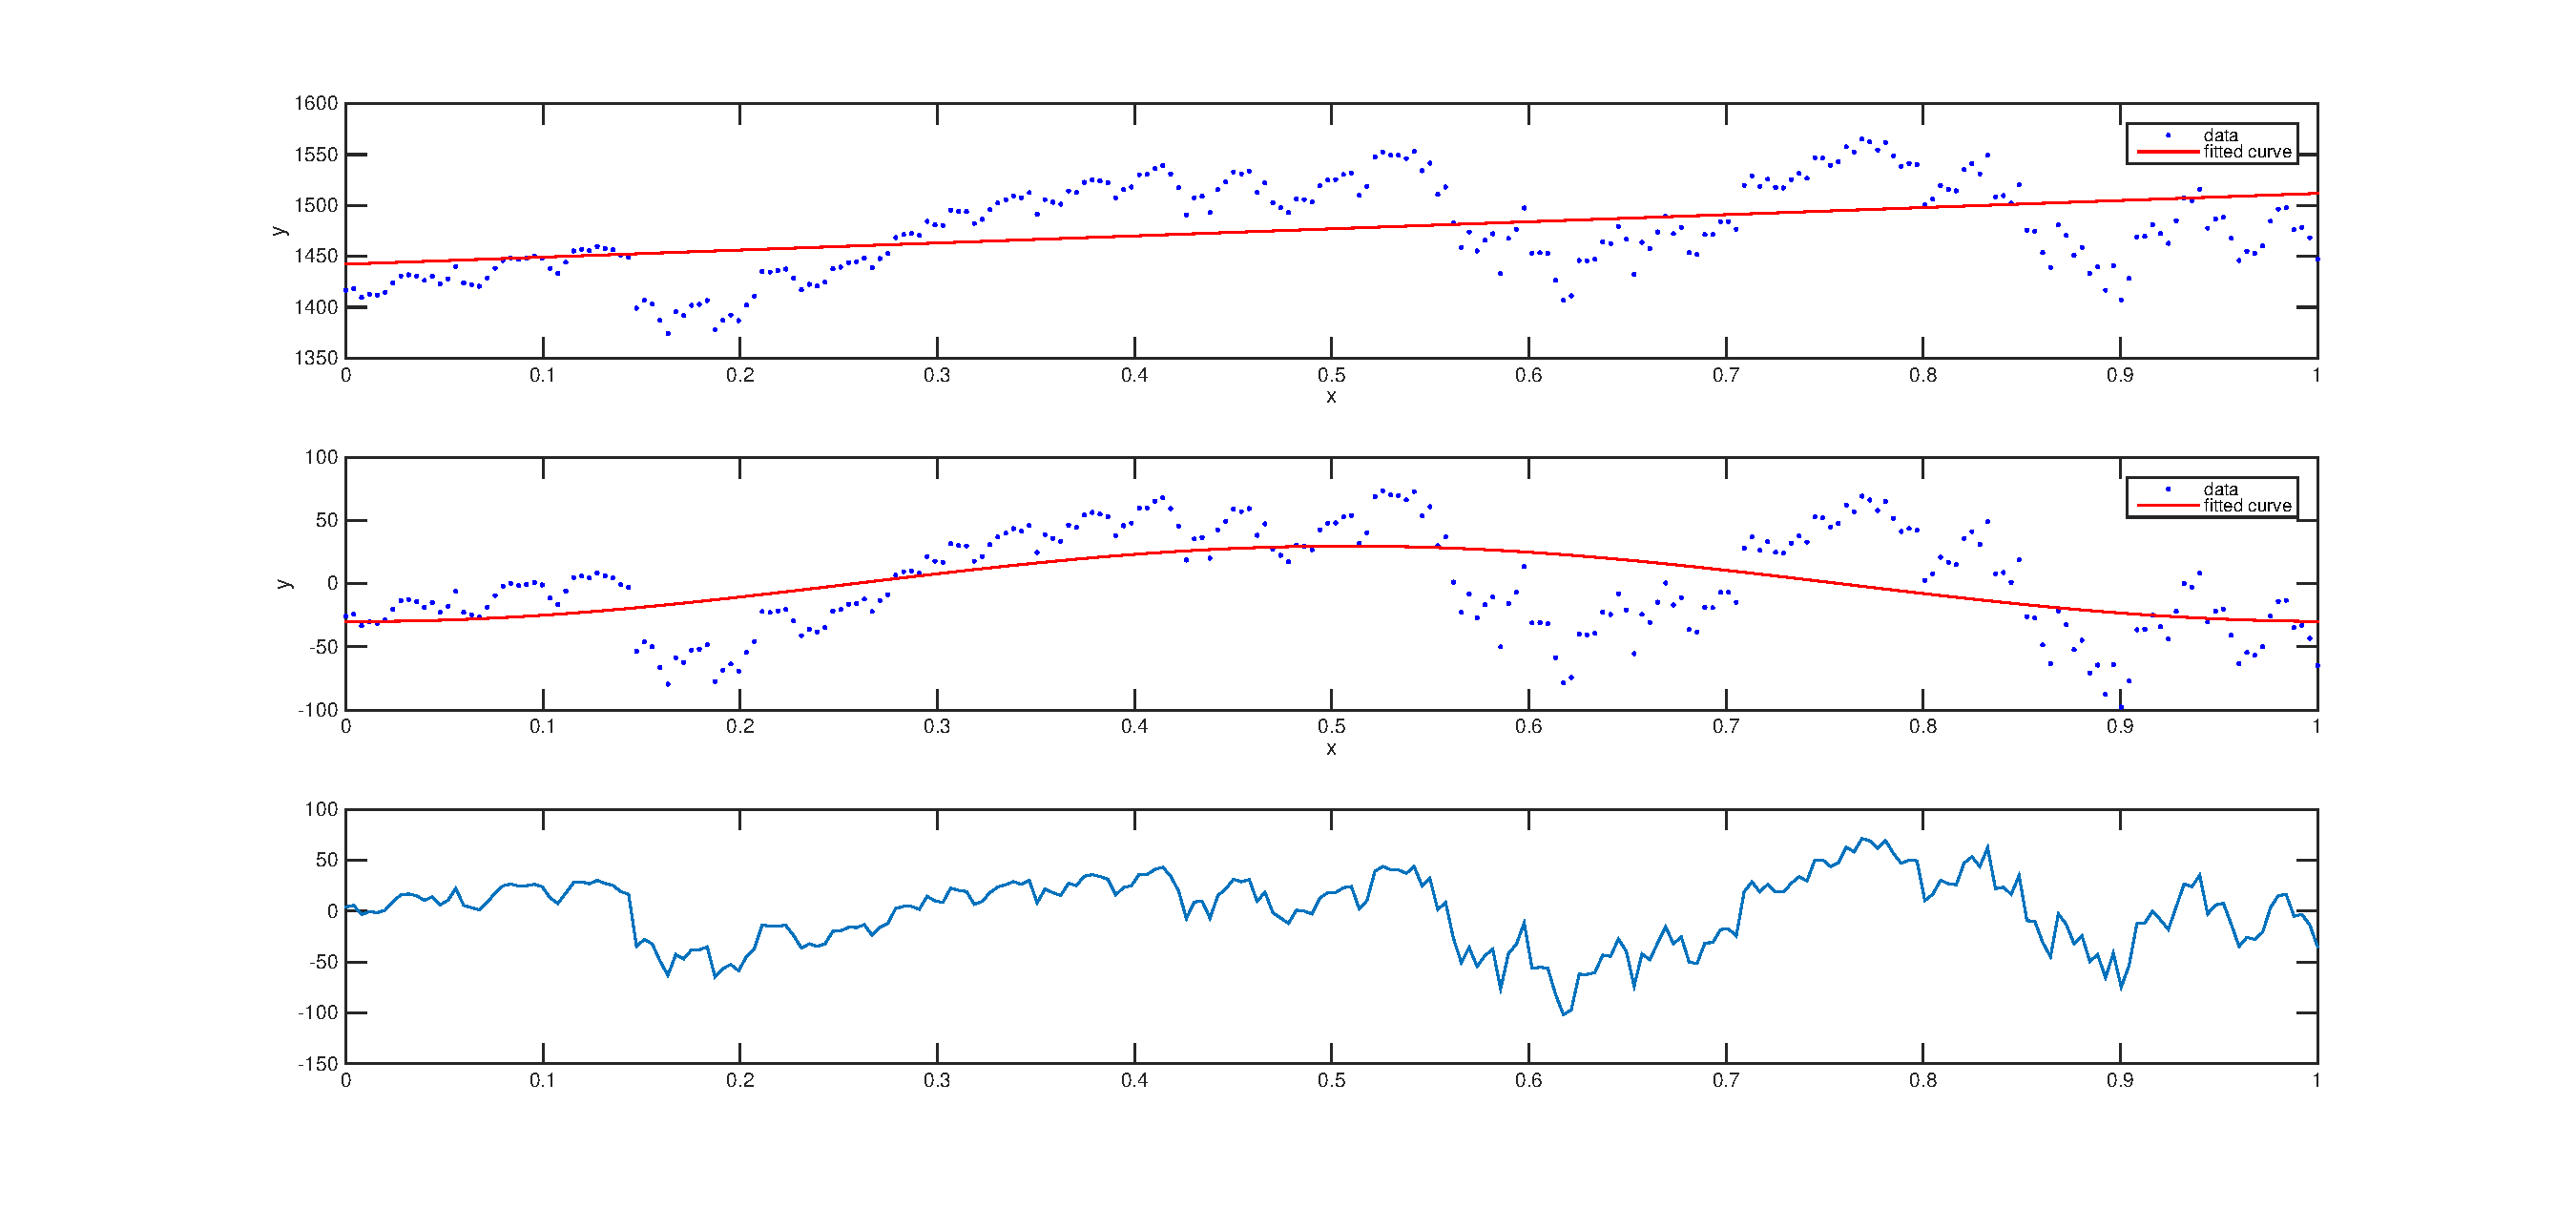
\includegraphics[width=\textwidth]{detrend.eps}

Next is the important part. In \cite{caete09}, the author also propose an indicator for predicting drawdowns in asset prices. For a given fixed time $t$ and a set of scales $S=\{1,\dots,N=2^k\}$, where $k\in \mathbb{N}$. The indicator $\zeta \in [0,1]$ is given by
\begin{equation}
\zeta(t) = \frac{card{\{ s \in S: W_f(t,s) > K\}}}{N}
\end{equation}

In practice asset price data are from a set of given time points $T = \{t_1,t_2,...,t_M\}$, so $K$ can be obtained by, for example, calculating an average of $\{ W_f(t,s)\}_{s\in S, t\in T}$. As for $N$ it is up to us to decide how many data points around time $t$ we want to included in the calculation of $W_f(t,s)$. This is because larger scales $s$ correspond to wider supports of $\psi^{t,s}$. It can be seen from (\ref{def:cwt}) that all of values $f(u)$ for which $u \in supp(\psi^{t,s})$ are needed when computing $W_f(t,s)$. Next figure illustrates the range of $f$ that is required in calculation of $W_f(50,4)$.

\includegraphics[width=\textwidth]{wavsupport.eps}

\section{My Experiment}

\subsection{Drawdown Detection, Batch Version}
Figure below is my attempt to replicate result in \cite{caete09}, which claims that $\zeta$ will rise to it peak before the start of soon coming drawdown. I obtain similar results on S\&P500, DAX, FTSE100 and NKY. My understanding is that price movement itself in all these four indexs are very close to each other. In the figure below a slightly modified version of $\zeta$ is shown in red, is compared with S\&P500 index.(Note that in the figure is my modified indicator whose range is [0,0.5] but later I discard that indicator and just work with $\zeta \in$ [0,1]). It can be seen that just before each drawdown start, it always climb to maximum of the range or just below that level. So it should be a good indicator. But one have to keep in mind that computation of $W_f(t,s)$ itself requires data from both future and past, which is not practical in live trading application.
\includegraphics[width=\textwidth]{drawdown.jpg}
\includegraphics[width=\textwidth]{pastvsfuture1.eps}

\newpage
\subsection{Drawdown Detection, Online Version}
In below figure, it is shown that once we allow less future data, the signal $\zeta$ degrade into a not very reliable signal. Also notice that by padding future five days data, the signal quality recovers to a degree that it might be working.
\includegraphics[width=\textwidth]{boundaryeffect.png}

\newpage
\subsection{Application on Volatility Swap}

From the observation in last subsection that 5 days more data might be enough to get a good approximation of $\zeta$ signal. My work on this section base on $\hat{\zeta}$ defined by
\begin{align}
\hat{\zeta}(t) &= \frac{card{\{ s \in S: W_{\hat{f}}(t-5,s) > K\}}}{N} \\
\hat{f}(u) &= \mathbb{I}_{u \leq t}, \forall u \nonumber
\end{align}
, given that current time is $t$.

The objective of my project is to aid decision about one month volatity swap. By starting taking the position today, the pay-off will be realized in the next 20 days, and it is equals to

\begin{align}
\texttt{Payoff}(t+20) = IV(t) -  RV(t+20)\\
RV(t+20) = \sqrt{\sum_{i=1}^{20} \frac{252}{20}\left(\log{\frac{P_{t+i}}{P_{t+i-1}}}\right)^2 } \nonumber
\end{align}
,and $IV(t)$ is an implied volatility on day $t$.

So it is helpful to look at how well $\hat{\zeta}$ can predict loss. I've found that $\hat{\zeta}$ leads $RV-IV$ by 10 days. And when $\hat{\zeta}$ was lagged by this number of days, two time series move together peak to peak
 
\includegraphics[width=\textwidth]{zetaleadspread.eps}

Being capable to predict ten days in advance is not particularly useful when the swap position must be taken 20 days before the strike. But by looking closely at lag 15, one can see that the correlation is still significant. To see in effect if this fact really does matter, one can also look at the table below. 


$$
E(IV(t-20)-RV(t) | \hat{\zeta}(t-15) > X)
$$

\begin{center}
\begin{tabular}{ |c|c|c| } 
 \hline
   X    &  days   &  AvgPayoff 	\\
 \hline
 0.000  &   1757  &    3.729	\\
 0.100  &   1713  &    3.687	\\
 0.200  &   1612  &    3.540	\\
 0.300  &   1446  &    3.322	\\
 0.400  &   1240  &    3.037	\\
 0.500  &    916  &    2.029	\\
 0.600  &    626  &    1.059	\\
 0.700  &    399  &    0.099	\\
 0.800  &    228  &   -1.106	\\
 0.900  &    131  &   -1.648	\\
 \hline
\end{tabular}
\end{center}


This is, again, cannot turn into useful indicator because 15 < 20. But it suggest

\begin{enumerate}
  \item Our approximate $\hat{\zeta}$ lags drawdown approximately by 5 days. 
  \item Above table tell that information we gain from $\hat{\zeta}$ can differentiate next 15 days average return of $RV-IV$. So this suggest that, in order to decide our position 20 days in advance, we must be able to accurately detect drawdown once it starts with as little delay as possible.
\end{enumerate}

\includegraphics[width=\textwidth]{linkdrawdownspread.eps}

Miscellaneous point to make is: the start of drawdowns always precede zetas, which, in turn, lead local maximas of spreads $RV-IV$ within the next 20 days but it does not tell if the spread will rise above zeros.


\begin{thebibliography}{1}
\bibitem{caete09} M.A.L Caetano; T.Yoneyama,CA: New indicator of imminent occurrence of drawdown in the stock market; In: Physica A, No. 388, 2009. pp. 3563-3571.
\end{thebibliography}

\end{document}